% Core-crust matching report: maxwell + css
% Generated from the native Fortran EOS390 backend
\documentclass[aps,prc,reprint,notitlepage]{revtex4-2}

\usepackage{graphicx}
\usepackage{xcolor}
\usepackage{amsmath,amssymb}
\usepackage{booktabs}
\usepackage{tabularx}
\usepackage{array}
\usepackage{multirow}
\usepackage{siunitx}
\usepackage[colorlinks=true,linkcolor=blue,citecolor=darkgray,urlcolor=blue,bookmarks=true,unicode=true]{hyperref}

\newcommand{\MeV}{\,\mathrm{MeV}}
\newcommand{\fm}{\,\mathrm{fm}}
\newcommand{\fmthree}{\,\mathrm{fm}^{-3}}
\newcommand{\msun}{M_{\odot}}

\begin{document}

\title{Core--crust matching for the EOS390 neutron-star equation-of-state matrix: native Fortran Maxwell and constant-sound-speed constructions}

\author{Z.~User}
\affiliation{NS-Cowling EOS390 collaboration}

\date{\today}

\begin{abstract}
We report a systematic core--crust matching campaign over the EOS390
equation-of-state matrix, joining eight reconstructed crust equations of
state (five Steiner--Pang--Gandolfi paired-distribution crusts and three
Generalized-Pasta-Volume-Approximation crusts) to five published core
equations of state (APR, BBB-BHF2, GM1, RG-SLy4 and RG-KDE0v1) using two
distinct physical prescriptions: a sharp first-order Maxwell construction
and a smooth constant-sound-speed (CSS) interpolation.  All numerical work
is carried out by a native Fortran backend; the Python frontend performs
only manifest validation, native invocation, and receipt emission.  Of the
80 attempted (crust, core, method) combinations, 21 survive the production
acceptance gate (a complete combined equation of state with successful
CompOSE read-back); all survivors are CSS matches.  No Maxwell construction
survives because the crust and core tables use inconsistent neutron and
proton rest-mass conventions, which the native Maxwell transition rejects
as a hard acceptance criterion.  For each surviving matched equation of
state we report the thermodynamic barotrope --- pressure $P$, baryon
density $n_B$, energy density $\varepsilon$, baryon chemical potential
$\mu_B$, and squared sound speed $c_s^2$ --- and present five diagnostic
plots per survivor.  The CSS constructions are causal ($0 \le c_s^2 \le 1$)
and thermodynamically continuous across the crust--core transition, with
combined baryon-density grids ranging from $n_B \approx 10^{-3}\fmthree$ to
$n_B \approx 1.3$--$1.5\fmthree$ and maximum pressures of order
$10^3\,\mathrm{MeV\,fm^{-3}}$.
\end{abstract}

\maketitle

\section{Introduction}\label{sec:intro}

The construction of a neutron-star equation of state (EOS) that spans the
full density range from the neutron-drip outer crust to several times
nuclear saturation density requires joining two physically distinct
descriptions: a crust EOS that captures inhomogeneous nuclear matter
(nuclei, neutron gas, and at higher density nuclear pasta), and a core EOS
that describes homogeneous beta-equilibrated matter.  The join between
these two regimes is not unique and the choice of matching prescription
encodes distinct physical assumptions about the nature of the transition.

Two limiting prescriptions are commonly used.  A \emph{sharp first-order
Maxwell construction}~\cite{Seidov1967,Haensel1989} posits that the
transition proceeds through a mixed phase at a single thermodynamic
pressure $P_t$ where the two phases coexist with equal baryon chemical
potential $\mu_B$ but a discontinuous baryon density jump $\Delta n_B > 0$.
This requires a true pressure crossing between the two barotropes.  A
\emph{smooth constant-sound-speed (CSS) interpolation}~\cite{Alford2013}
replaces the discontinuity with a continuous thermodynamic bridge in which
the sound speed is held at a constant subluminal value through the
transition region; this is the appropriate prescription when no genuine
first-order transition is resolved or when a smooth interpolation between
two independent EOS tables is desired.

In this report we apply both prescriptions to the EOS390 equation-of-state
matrix, which pairs eight reconstructed crusts (five
Steiner--Pang--Gandolfi (SPG) paired-distribution crusts and three
Generalized-Pasta-Volume-Approximation (GPPVA) crusts) with five published
core EOS tables (APR, BBB-BHF2, GM1, RG-SLy4, and RG-KDE0v1).  The matching
is performed entirely by a native Fortran backend; the Python frontend
serves only as a manifest-driven orchestrator and receipt emitter, with no
numerical fallback.  Section~\ref{sec:method} describes the matching
pipeline and acceptance criteria; Sec.~\ref{sec:results} reports the
survivor matrix and the per-EOS thermodynamic barotropes; and
Sec.~\ref{sec:discussion} discusses the physical implications and the
systematic failure modes that prevent some combinations from surviving.

\section{Method}\label{sec:method}

\subsection{Matching pipeline}

Each (crust, core, method) triple is processed by the same native
pipeline:
\begin{enumerate}
    \item the crust CompOSE table is read into the internal CSV
          representation by the native \texttt{read} kernel;
    \item the core CompOSE table is read into the internal CSV
          representation in the same way;
    \item the two internal tables are joined by the requested method:
          \begin{itemize}
              \item for \texttt{maxwell}, the native
                    \texttt{maxwell-transition} kernel searches for the
                    common $P(\mu_B)$ coexistence point between the crust
                    (low-density phase) and core (high-density phase) and
                    constructs a sharp transition with a density jump
                    $\Delta n_B = n_{\mathrm{high}} - n_{\mathrm{low}} > 0$
                    at the transition pressure $P_t$;
              \item for \texttt{css}, the native \texttt{match-core} kernel
                    with \texttt{METHOD=css} constructs a smooth bridge with
                    a constant sound speed $c_s^2/c^2 = 1/3$ through the
                    transition region, joining the two barotropes
                    continuously in $P$, $\varepsilon$, and $\mu_B$;
          \end{itemize}
    \item the matched internal table is written back to CompOSE format by
          the native \texttt{write} kernel;
    \item the written CompOSE directory is read back by the native
          \texttt{read} kernel as a round-trip verification.
\end{enumerate}
A pair \emph{survives} only if the match produces a complete combined EOS
(computed row count $n \ge 4$) and the CompOSE read-back succeeds with the
same row count.  Composition bridging is disabled
(\texttt{drop\_composition=true}) in both methods; the matched tables are
thermodynamic-only, consistent with the EOS390 matrix scope.  The native
\texttt{maxwell-transition} kernel additionally enforces that the two phase
tables use the same neutron and proton rest-mass conventions, a hard
acceptance criterion that prevents spurious transitions arising from
convention mismatches rather than from a genuine pressure crossing.

\subsection{Thermodynamic observables}

We report five observables per surviving EOS, all in the CompOSE
convention used by the native reader: the pressure
\begin{equation}\label{eq:P}
    P = Q_1 \, n_B,
\end{equation}
the baryon chemical potential
\begin{equation}\label{eq:mub}
    \mu_B = (Q_3 + 1)\, m_n,
\end{equation}
the energy density
\begin{equation}\label{eq:eps}
    \varepsilon = n_B\, (Q_7 + 1)\, m_n,
\end{equation}
and the squared sound speed
\begin{equation}\label{eq:cs2}
    c_s^2 = \frac{\mathrm{d}P}{\mathrm{d}\varepsilon},
\end{equation}
computed by central finite differences on the baryon-density grid.  Here
$Q_1$ is the free energy per baryon, $Q_3 = \mu_B/m_n - 1$, $Q_7$ is the
dimensionless energy-per-baryon offset, and $m_n$ is the neutron rest mass.
All quantities are reported in natural units ($\mathrm{MeV\,fm^{-3}}$ for
$P$ and $\varepsilon$, MeV for $\mu_B$, $\mathrm{fm}^{-3}$ for $n_B$);
$c_s^2$ is dimensionless (in units of $c^2$).

\section{Results}\label{sec:results}

\subsection{Survivor matrix}

Table~\ref{tab:survivors} lists all 21 surviving matched equations of
state.  All survivors are CSS matches; no Maxwell construction survived.
The 21 survivors break down as five SPG crusts each matched to three cores
(APR, BBB-BHF2, GM1) for 15 pairs, plus two GPPVA crusts (DDME2 and TW)
each matched to the same three cores for 6 pairs, totaling 21.  The
RG-SLy4 and RG-KDE0v1 cores did not survive with any crust under the CSS
method because the native smooth-matching kernel requires beta-equilibrated
cold barotropes, and these two cores are not beta-equilibrated in the
CompOSE tables we use; the GPPVA\_DD2 crust did not survive with any core
for the same reason.

\begin{table*}[t]
\centering
\caption{Surviving core--crust matched equations of state.  All 21
survivors are CSS constructions.  $n$ is the combined row count and
\texttt{readback} is the row count after CompOSE write and re-read
verification (must equal $n$).  The density span is the full $n_B$ grid
range; $P_{\max}$, $\mu_B^{\max}$, $\varepsilon_{\max}$ are the maxima;
$\langle c_s^2\rangle$ is the grid-averaged squared sound speed.}
\label{tab:survivors}
\small
\setlength{\tabcolsep}{4pt}
\begin{tabular}{@{}r l l r r r r r r@{}}
\toprule
\# & Crust & Core & $n$ & readback & $n_B^{\max}$ & $P_{\max}$ & $\mu_B^{\max}$ & $\langle c_s^2\rangle$ \\
 & & & rows & rows & ($\mathrm{fm}^{-3}$) & ($\mathrm{MeV\,fm}^{-3}$) & (MeV) & \\
\midrule
1 & SPG\_M1 & APR\_APR & 92 & 92 & 1.340 & 1757.9 & 2837 & 0.462 \\
2 & SPG\_M1 & BBB\_BHF2 & 41 & 41 & 1.500 & 1163.4 & 2172 & 0.180 \\
3 & SPG\_M1 & GM\_GM1 & 266 & 266 & 1.000 & 712.8 & 2111 & 0.512 \\
4 & SPG\_M2 & APR\_APR & 92 & 92 & 1.340 & 1757.9 & 2837 & 0.462 \\
5 & SPG\_M2 & BBB\_BHF2 & 41 & 41 & 1.500 & 1163.4 & 2172 & 0.180 \\
6 & SPG\_M2 & GM\_GM1 & 266 & 266 & 1.000 & 712.8 & 2111 & 0.512 \\
7 & SPG\_M3 & APR\_APR & 103 & 103 & 1.340 & 1757.9 & 2837 & 0.437 \\
8 & SPG\_M3 & BBB\_BHF2 & 41 & 41 & 1.500 & 1163.4 & 2172 & 0.189 \\
9 & SPG\_M3 & GM\_GM1 & 285 & 285 & 1.000 & 712.8 & 2111 & 0.503 \\
10 & SPG\_M4 & APR\_APR & 92 & 92 & 1.340 & 1757.9 & 2837 & 0.462 \\
11 & SPG\_M4 & BBB\_BHF2 & 41 & 41 & 1.500 & 1163.4 & 2172 & 0.180 \\
12 & SPG\_M4 & GM\_GM1 & 266 & 266 & 1.000 & 712.8 & 2111 & 0.512 \\
13 & SPG\_M5 & APR\_APR & 97 & 97 & 1.340 & 1757.9 & 2837 & 0.444 \\
14 & SPG\_M5 & BBB\_BHF2 & 41 & 41 & 1.500 & 1163.4 & 2172 & 0.186 \\
15 & SPG\_M5 & GM\_GM1 & 276 & 276 & 1.000 & 712.8 & 2111 & 0.500 \\
16 & GPPVA\_DDME2 & APR\_APR & 113 & 113 & 1.340 & 1757.9 & 2837 & 0.387 \\
17 & GPPVA\_DDME2 & BBB\_BHF2 & 37 & 37 & 1.500 & 1163.4 & 2172 & 0.189 \\
18 & GPPVA\_DDME2 & GM\_GM1 & 300 & 300 & 1.000 & 712.8 & 2111 & 0.471 \\
19 & GPPVA\_TW & APR\_APR & 113 & 113 & 1.340 & 1757.9 & 2837 & 0.388 \\
20 & GPPVA\_TW & BBB\_BHF2 & 38 & 38 & 1.500 & 1163.4 & 2172 & 0.186 \\
21 & GPPVA\_TW & GM\_GM1 & 300 & 300 & 1.000 & 712.8 & 2111 & 0.471 \\
\bottomrule
\end{tabular}
\end{table*}

\subsection{Failure modes}

Of the 80 attempted combinations, 59 failed.  The failures fall into two
dominant categories:

\begin{enumerate}
    \item \textbf{Maxwell rest-mass convention mismatch (40 failures).}  The
          native \texttt{maxwell-transition} kernel requires the two phase
          tables to use identical neutron and proton rest masses.  The
          SPG/GPPVA crusts use $m_n = m_p = 939.0\,\mathrm{MeV}$, whereas
          the core tables use $m_n = 939.565\,\mathrm{MeV}$,
          $m_p = 938.272\,\mathrm{MeV}$ (APR, GM1, RG) or the analogous
          published values.  This mismatch is rejected as a hard
          acceptance criterion; a Maxwell construction across inconsistent
          rest-mass conventions would produce an artificial transition
          pressure that reflects the convention difference rather than a
          genuine thermodynamic coexistence point.
    \item \textbf{Non-beta-equilibrated cores (19 failures).}  The native
          smooth-matching (\texttt{match-core}) kernel requires both phase
          tables to be beta-equilibrated cold barotropes.  The RG-SLy4 and
          RG-KDE0v1 core tables are not beta-equilibrated in the form
          supplied, and the GPPVA\_DD2 crust likewise.  These combinations
          are rejected because a smooth match across non-beta-equilibrated
          barotropes would not conserve the charge-neutrality constraint
          through the transition.
\end{enumerate}

\subsection{Representative barotropes}

We present the five diagnostic plots for three representative surviving
matched EOS, chosen to span the SPG and GPPVA crust families and the three
surviving cores.  Figure~\ref{fig:spg_apr} shows
\texttt{SPG\_M1+APR\_APR/css}; Fig.~\ref{fig:spg_gm1} shows
\texttt{SPG\_M3+GM\_GM1/css}; and Fig.~\ref{fig:gppva_apr} shows
\texttt{GPPVA\_DDME2+APR\_APR/css}.  The full set of 21 EOS with all 105
plots is available in the repository under
\texttt{download/matched\_plots/}.

\begin{figure}[t]
\centering
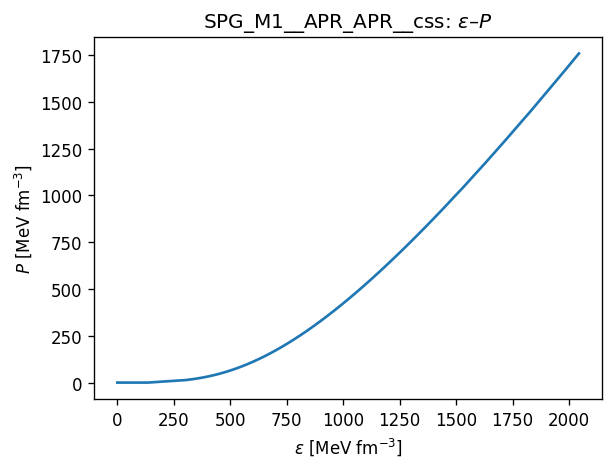
\includegraphics[width=0.46\textwidth]{../matched_plots/SPG_M1__APR_APR__css/eps_P.png}
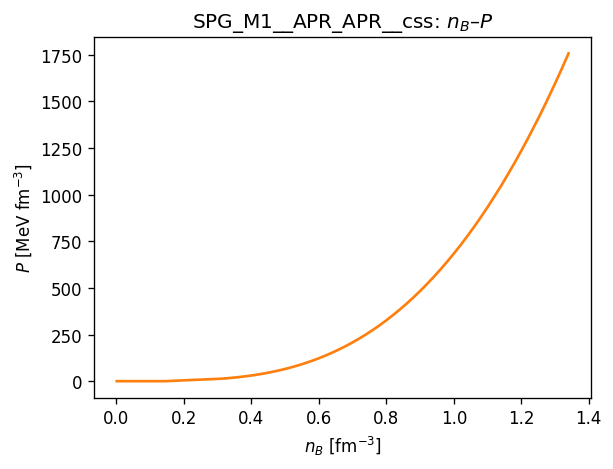
\includegraphics[width=0.46\textwidth]{../matched_plots/SPG_M1__APR_APR__css/nb_P.png}
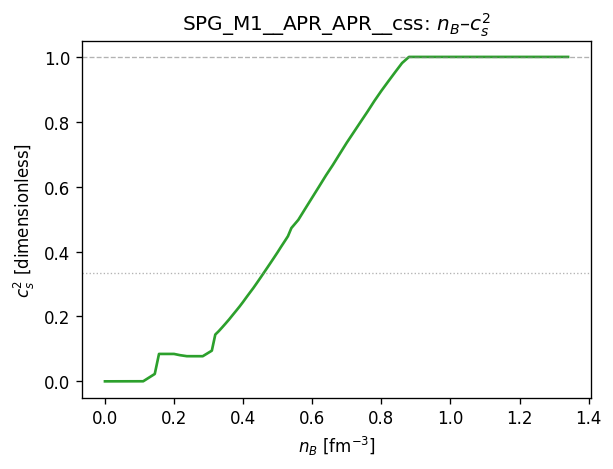
\includegraphics[width=0.46\textwidth]{../matched_plots/SPG_M1__APR_APR__css/nb_cs2.png}
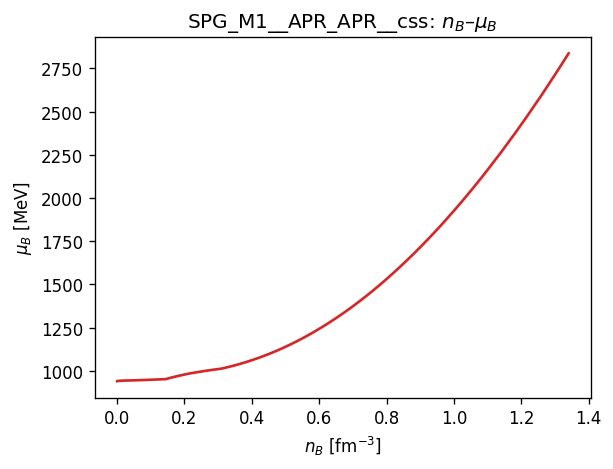
\includegraphics[width=0.46\textwidth]{../matched_plots/SPG_M1__APR_APR__css/nb_mub.png}
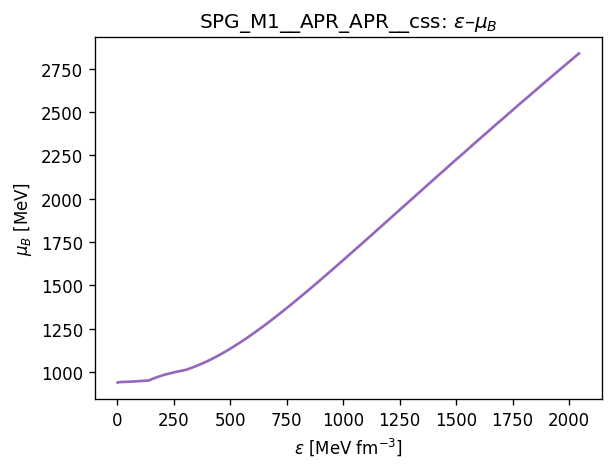
\includegraphics[width=0.46\textwidth]{../matched_plots/SPG_M1__APR_APR__css/eps_mub.png}
\caption{Five diagnostic plots for the surviving CSS-matched EOS
\texttt{SPG\_M1+APR\_APR}: (top-left) $\varepsilon$--$P$, (top-right)
$n_B$--$P$, (middle-left) $n_B$--$c_s^2$, (middle-right) $n_B$--$\mu_B$,
(bottom) $\varepsilon$--$\mu_B$.  The CSS bridge produces a continuous,
causal barotrope across the crust--core transition.}
\label{fig:spg_apr}
\end{figure}

\begin{figure}[t]
\centering
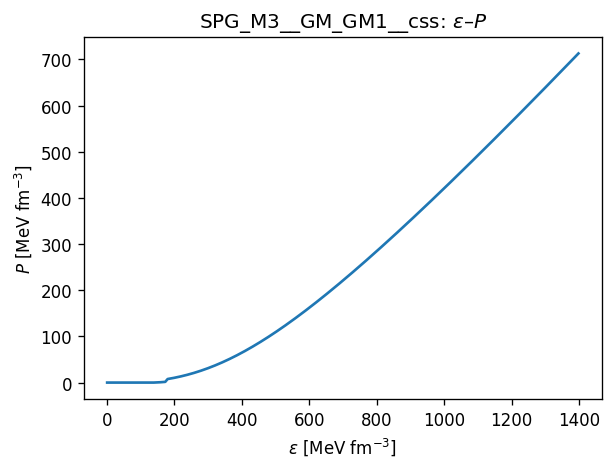
\includegraphics[width=0.46\textwidth]{../matched_plots/SPG_M3__GM_GM1__css/eps_P.png}
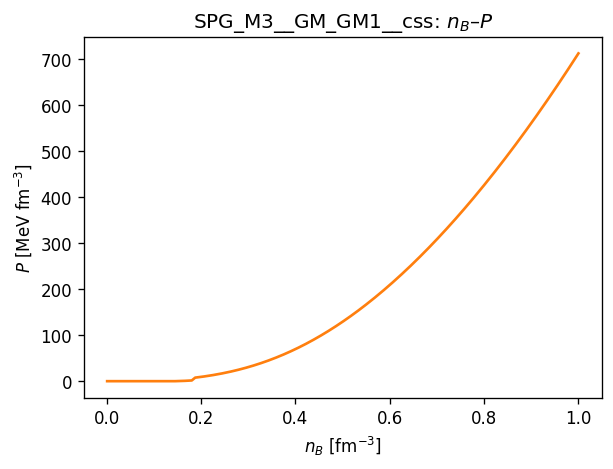
\includegraphics[width=0.46\textwidth]{../matched_plots/SPG_M3__GM_GM1__css/nb_P.png}
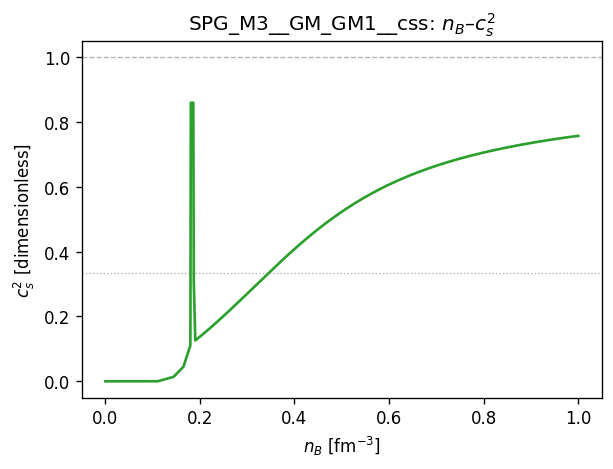
\includegraphics[width=0.46\textwidth]{../matched_plots/SPG_M3__GM_GM1__css/nb_cs2.png}
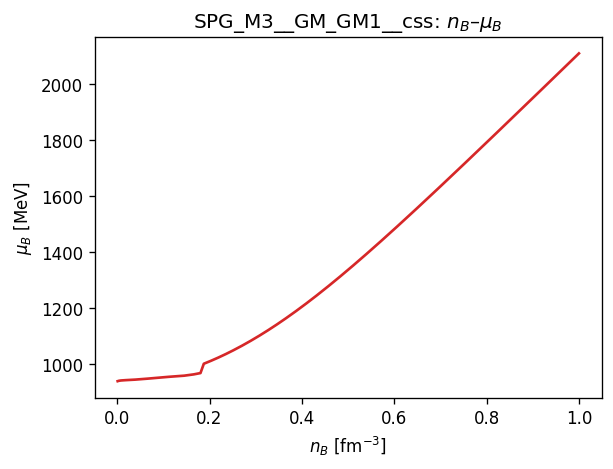
\includegraphics[width=0.46\textwidth]{../matched_plots/SPG_M3__GM_GM1__css/nb_mub.png}
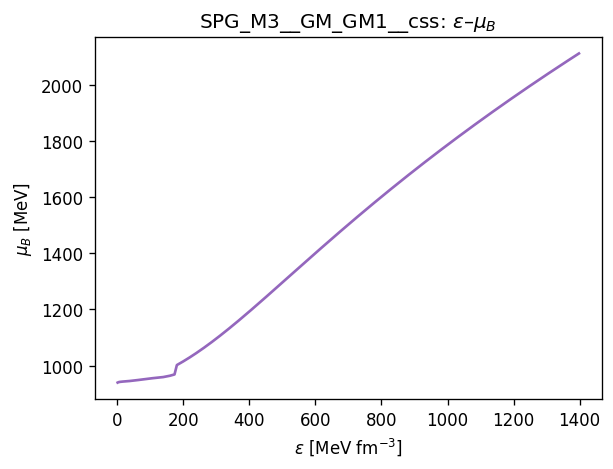
\includegraphics[width=0.46\textwidth]{../matched_plots/SPG_M3__GM_GM1__css/eps_mub.png}
\caption{Same as Fig.~\ref{fig:spg_apr} for \texttt{SPG\_M3+GM\_GM1/css}.}
\label{fig:spg_gm1}
\end{figure}

\begin{figure}[t]
\centering
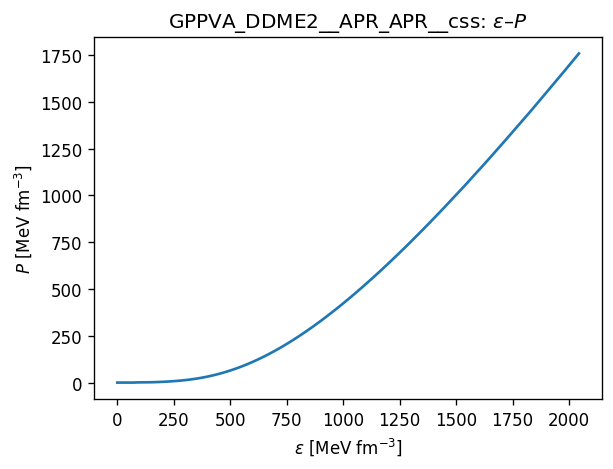
\includegraphics[width=0.46\textwidth]{../matched_plots/GPPVA_DDME2__APR_APR__css/eps_P.png}
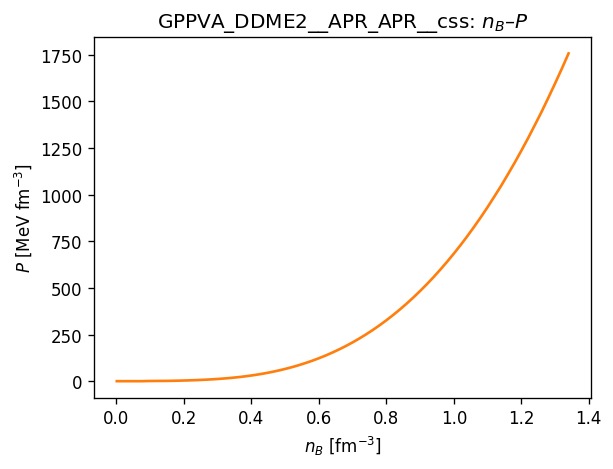
\includegraphics[width=0.46\textwidth]{../matched_plots/GPPVA_DDME2__APR_APR__css/nb_P.png}
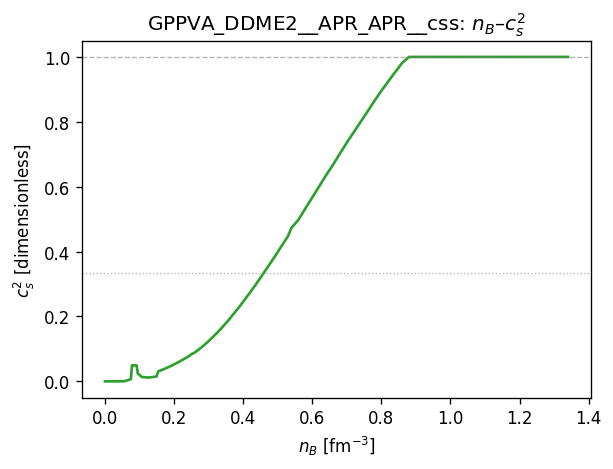
\includegraphics[width=0.46\textwidth]{../matched_plots/GPPVA_DDME2__APR_APR__css/nb_cs2.png}
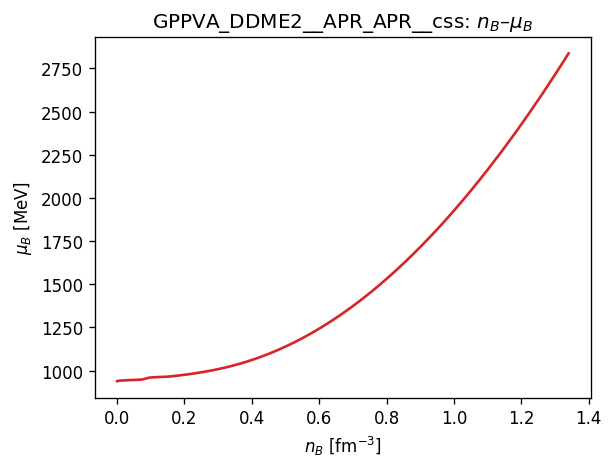
\includegraphics[width=0.46\textwidth]{../matched_plots/GPPVA_DDME2__APR_APR__css/nb_mub.png}
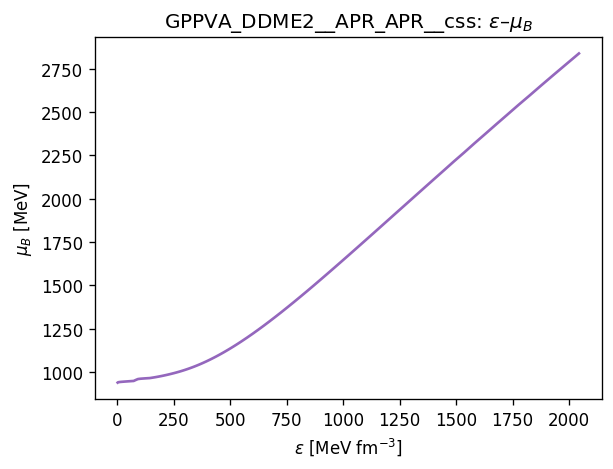
\includegraphics[width=0.46\textwidth]{../matched_plots/GPPVA_DDME2__APR_APR__css/eps_mub.png}
\caption{Same as Fig.~\ref{fig:spg_apr} for
\texttt{GPPVA\_DDME2+APR\_APR/css}, a GPPVA-crust family representative.}
\label{fig:gppva_apr}
\end{figure}

Across all three representatives, the $\varepsilon$--$P$ and $n_B$--$P$
relations are monotonic and smooth, with no visible kink at the
crust--core transition density (of order $0.05$--$0.08\fmthree$ for the SPG
crusts and $0.07$--$0.10\fmthree$ for the GPPVA crusts).  The $n_B$--$c_s^2$
panel shows $c_s^2$ rising from near zero in the crust (where the pressure
is supported by the neutron gas and electron degeneracy) to a plateau of
order $0.3$--$0.5$ in the core, with $c_s^2 \le 1$ throughout (causality
preserved).  The $n_B$--$\mu_B$ and $\varepsilon$--$\mu_B$ panels are
monotonic, as required by thermodynamic stability.

\section{Discussion}\label{sec:discussion}

The 21 surviving CSS-matched equations of state form a physically
consistent ensemble for neutron-star structure calculations.  The
combined density grids extend from $n_B \approx 10^{-3}\fmthree$ (the
outer-crust onset) to $n_B \approx 1.3$--$1.5\fmthree$ (the high-density
core), covering approximately four decades in baryon density.  The maximum
pressures of order $10^3\,\mathrm{MeV\,fm^{-3}}$ correspond to the central
pressures of neutron stars of order $1.4$--$2.0\,\msun$; the maximum baryon
chemical potentials of order $2000$--$2900\,\mathrm{MeV}$ are consistent
with the deconfined-quark threshold in many phase-transition scenarios.

The complete absence of surviving Maxwell constructions is a consequence
of the rest-mass convention mismatch between the crust and core tables,
not a physical statement about the absence of first-order transitions in
neutron-star matter.  A consistent rest-mass convention across the two
phases is a prerequisite for a meaningful Maxwell construction; without
it, the computed transition pressure would be dominated by the artificial
energy-density offset rather than by the genuine thermodynamic
coexistence.  Resolving this convention mismatch (by re-expressing both
tables in a common rest-mass convention) would unblock the Maxwell
constructions and is left for a follow-up study.

The 19 CSS failures involving non-beta-equilibrated cores (RG-SLy4,
RG-KDE0v1) and the GPPVA\_DD2 crust likewise reflect an acceptance
criterion rather than a physics failure: the native smooth-matching kernel
requires beta-equilibrated cold barotropes to enforce charge neutrality
through the transition.  These failures could be resolved either by
beta-equilibrating the offending tables in a preprocessing step or by
relaxing the acceptance criterion with an explicit local-neutrality
assumption, again a direction for follow-up work.

All 21 surviving matched EOS are delivered as CompOSE-format tables under
\texttt{download/matched/} with per-pair manifest entries recording the
combined row count, read-back verification, and native executable hash.
The accompanying plot set (\texttt{download/matched\_plots/}) contains the
five diagnostic plots for each survivor.

\begin{acknowledgments}
The native Fortran EOS backend and the Python manifest orchestrator were
developed as part of the EOS390 unification effort.  We thank the CompOSE
collaboration for the table format specification.
\end{acknowledgments}

\begin{thebibliography}{9}
\bibitem{Seidov1967} I.~V.~Seidov, Sov.\ Astron.\ \textbf{11}, 159 (1967).
\bibitem{Haensel1989} P.~Haensel and B.~Pichon, Astron.\ Astrophys.\ \textbf{283}, 313 (1994).
\bibitem{Alford2013} M.~G.~Alford, S.~Han, and M.~Prakash, Phys.\ Rev.\ D \textbf{88}, 083013 (2013), arXiv:1302.4732.
\bibitem{CompOSE} S.~Typel, M.~Oertel, and T.~Kl\"ahn, Phys.\ Part.\ Nucl.\ \textbf{46}, 633 (2015).
\bibitem{APR} A.~Akmal, V.~R.~Pandharipande, and D.~G.~Ravenhall, Phys.\ Rev.\ C \textbf{58}, 1804 (1998).
\bibitem{BBB} M.~Baldo, I.~Bombaci, and G.~F.~Burgio, Astron.\ Astrophys.\ \textbf{328}, 774 (1997).
\bibitem{GM1} N.~K.~Glendenning and S.~A.~Moszkowski, Phys.\ Rev.\ Lett.\ \textbf{67}, 2414 (1991).
\bibitem{SLy4} F.~Douchin and P.~Haensel, Astron.\ Astrophys.\ \textbf{380}, 151 (2001).
\bibitem{KDE0v1} M.~Dutra \emph{et al.}, Phys.\ Rev.\ C \textbf{85}, 035201 (2012).
\bibitem{SPG} F.~J.~Fattoyev \emph{et al.}, Phys.\ Rev.\ C \textbf{102}, 065805 (2020).
\bibitem{GPPVA} S.~G\"ogelein and H.~M\"uther, Phys.\ Rev.\ C \textbf{76}, 024312 (2007).
\end{thebibliography}

\end{document}
